\documentclass[11pt, oneside]{article}   	% use "amsart" instead of "article" for AMSLaTeX format
\usepackage{geometry}                		% See geometry.pdf to learn the layout options. There are lots.
\geometry{letterpaper}                   		% ... or a4paper or a5paper or ... 
%\geometry{landscape}                		% Activate for for rotated page geometry
%\usepackage[parfill]{parskip}    		% Activate to begin paragraphs with an empty line rather than an indent
\usepackage{graphicx}				% Use pdf, png, jpg, or eps with pdflatex; use eps in DVI mode
								% TeX will automatically convert eps --> pdf in pdflatex		
\usepackage{xspace}
\usepackage{amssymb}
\usepackage{cite}

\usepackage{xcolor}
\usepackage{xspace}
\def\osprey{{\sc{osprey}}\xspace}

\usepackage{listings}
\lstset{
	basicstyle=\footnotesize
}

\newcommand{\jj}[1]{\if\submissionMode0{\em\color{blue}(JJ: #1)}\else\fi}
\newcommand{\jeff}[1]{\if\submissionMode0{\em\color{blue}(Jeff: #1)}\else\fi}
\newcommand{\suggestion}[1]{\if\submissionMode0{\color{green}\textbf{#1}}\else\fi}


%Submission guidelines for PLoS ONE: http://journals.plos.org/plosone/s/submission-guidelines

\title{{\sc osprey} 3: Open-Source Protein Redesign for You, Refactored, with Powerful New Features}
\author{Donald Lab}
%\date{}							% Activate to display a given date or no date

\begin{document}
\maketitle
%\section{}
%\subsection{}

\section{Abstract}

\section{Introduction}
For over a decade, the {\sc osprey} software package~\cite{OSPREY_MIE,minDEE,OSPREY_MIE,OSPREY} has offered the protein design community a unique combination of continuous flexibility modeling, ensemble modeling, and algorithms with provable guarantees~\cite{alg_SMB_textbook,cosb_design}.  Having begun as a software release for the $K^*$ algorithm~\cite{minDEE,GrsA-LeuA}, which approximates binding constants using ensemble modeling, it now boasts a wide array of algorithms found in no other software.  {\sc osprey} has been used in many designs that were empirically successful---\textit{in vitro}~\cite{VRC07_enhance,CFTR,runx1_cbfb,GrsA-LeuA,DHFR-PNAS,GrsA-TyrA,specific_probes} and \textit{in vivo}~\cite{VRC07_enhance,CFTR,runx1_cbfb,DHFR-PNAS} as well as in non-human primates~\cite{VRC07_enhance}.  {\sc osprey}'s predictions have been validated by a wide range of experimental methods, including binding assays, enzyme kinetics and activity assays, in cell assays (MICs, fitness) and viral neutralization, {\em in vivo} studies, and crystal~\cite{DHFR-PNAS2, VRC07_enhance} and NMR~\cite{runx1_cbfb} structures.    

However, as {\sc osprey} grew to include more algorithms and features (Fig.~\ref{flowchart}), the code became increasingly complicated and difficult to maintain.  The growing complexity of the software also hindered its ease-of-use. {\sc osprey} 3.0 represents a complete refactoring of the code, and presents a simpler and more intuitive interface that makes protein redesign much easier than before. The new, developer-friendly code organization also facilitates adding new features to the free and open-source \osprey project, both by ourselves and by other contributors.  We have introduced a convenient Python scripting interface and added support for GPU acceleration of the bulk of the computation, allowing designs to be completed much more quickly and easily than in previous versions of {\sc osprey}.  We believe {\sc osprey} 3.0 will be a very useful tool for both developers and users of provably accurate protein design algorithms.  


\begin{figure}
\center
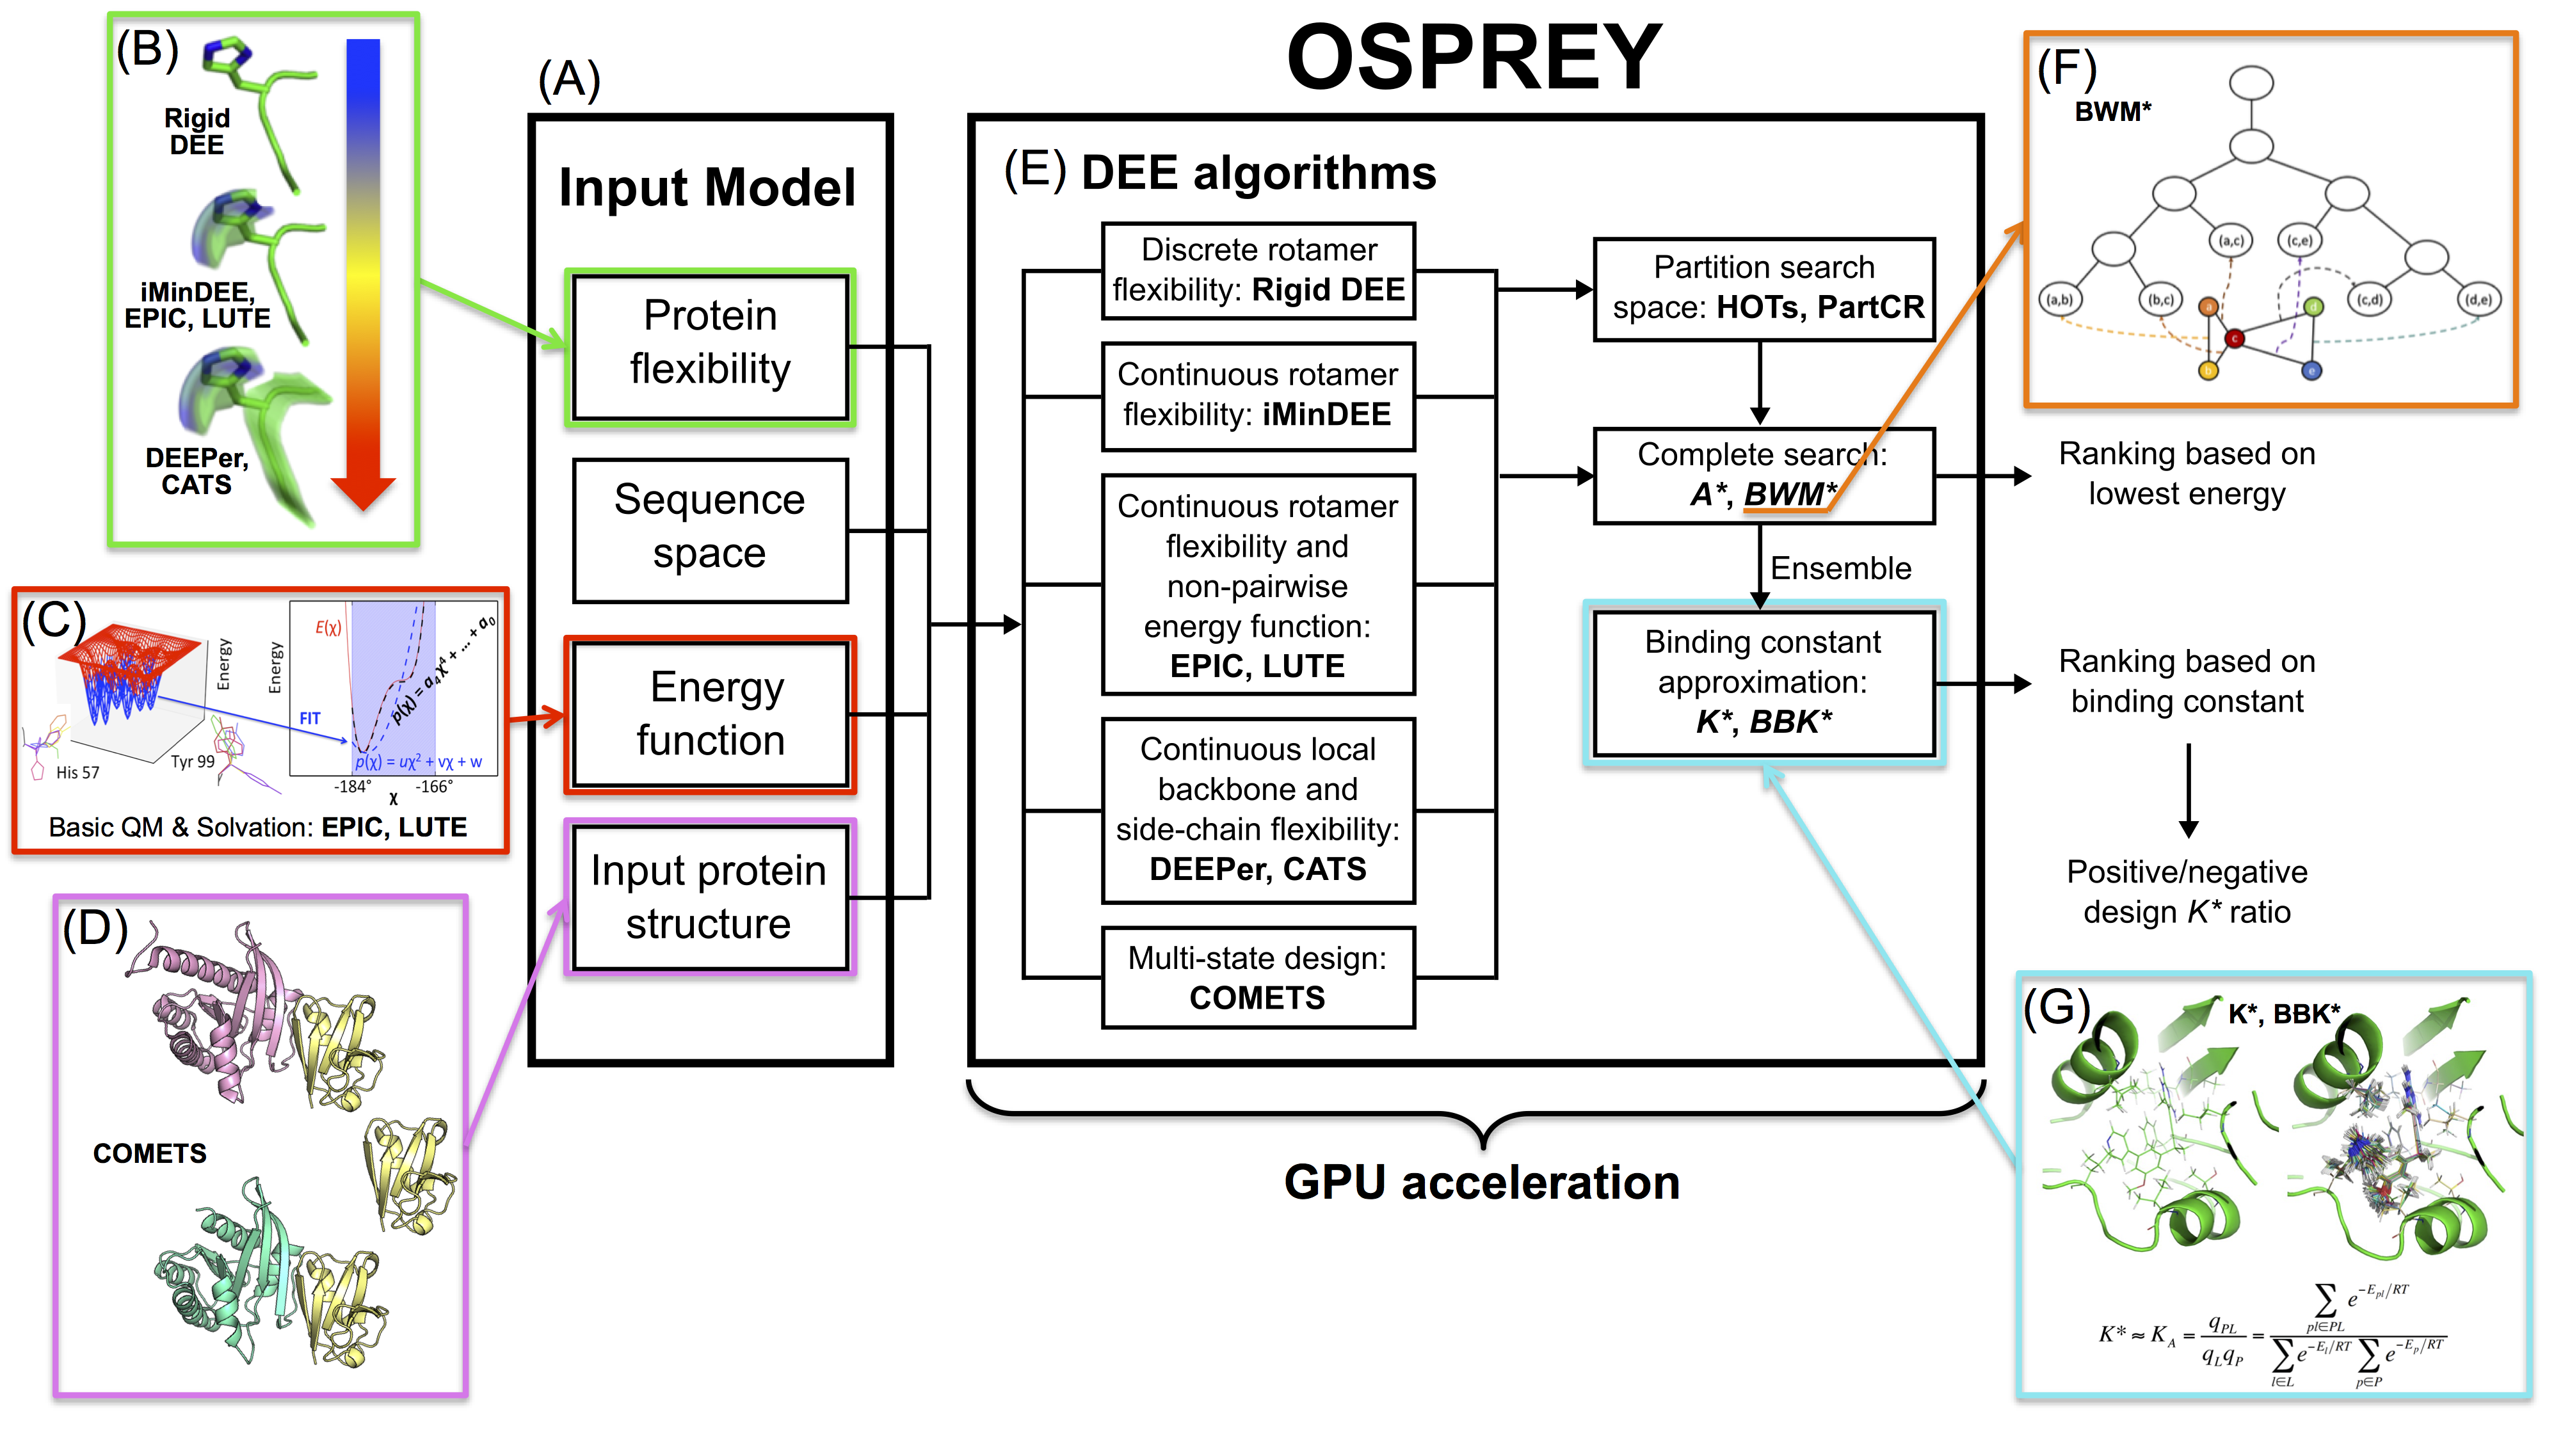
\includegraphics[width=6in]{figures/osprey_mantra.png}
 \vspace{-0.3in}%to fit the figure on one page
\caption{The \osprey protein redesign suite. (A) The input model includes a 3D structure of the protein to be redesigned, a definition of the sequence space, the allowed protein flexibility (including the rotamer library), and a pairwise energy function. (B) Rigid DEE~\cite{DEE,DEE/A*}, iMinDEE~\cite{iMinDEE}, EPIC~\cite{EPIC}, LUTE~\cite{LUTE_RECOMB}, DEEPer~\cite{DEEPer}, and CATS~\cite{CATS} model different types of protein flexibility. Flexibility ranges in difficulty from complete rigidity to continuous side chain flexibility to complete flexibility including continuous backbone flexibility. (C) The EPIC~\cite{EPIC} and LUTE~\cite{LUTE_RECOMB} algorithms also expand energy function capability by allowing for non-pairwise, basic QM and solvation. (D) COMETS~\cite{COMETS} allows for multi-state design by comparing various bound and unbound states. This allows for multiple input structures. (E) These algorithms are implemented in OSPREY and improved through the use of GPU acceleration. According to the allowed flexibility, OSPREY runs a specific pruning algorithm followed by the \as search algorithm. The \as output generates a ranking based on either the lowest-energy structure of each sequence, or an ensemble of structures computed by the \ks algorithm. (F) The \bwmstar~\cite{BWM*} algorithm takes advantage of sparse trees and branch decomposition to outperform traditional \as. (G) The \ks~\cite{K*,minDEE} algorithm calculates a \ks score (an approximation of the binding constant, $K_a$) by provably estimating the partition function for the protein, the ligand, and the protein-ligand complex. The \ks algorithm exploits a thermodynamic ensemble of structures as opposed to a single structure as illustrated in the panel (PDB ID: 3FQC). \ks can also be used to find sequences that have a high affinity for one ligand (positive design) while having a low affinity for another (negative design) by taking a ratio of \ks scores~\cite{DHFR-PNAS,DHFR-PNAS2}. }
\label{flowchart}
\end{figure}

\jccsubsection{Past successes of {\sc osprey}}

{\sc osprey} has been used for an impressive number of empirically successful designs, ranging from enzyme design to antibody design to prediction of antibiotic resistance mutations.  Notably, {\sc osprey} has been successful in many~\textit{prospective} experimental studies, i.e., studies in which our designed sequences are tested experimentally, thus validating \osprey through use in practice rather than simply through a retrospective comparison of OSPREY calculations to previous experimental results.  {\sc osprey} is most applicable to problems that can be posed in terms of biophysical state transitions like binding, allowing the $K^*$ algorithm and its variants to predict the optimal sequences based on an estimate of binding free energy computed using Boltzmann-weighted conformational ensembles.  Moreover, most protein design problems can be posed in this way, sometimes in terms of binding to more than one ligand.  \osprey is capable of both~\textit{positive design}, in which binding of a designed protein to a target is increased, and~\textit{negative design}, in which binding to a target is decreased, as well as more complicated design objectives where specific binding to one target and not to another is required.  

For example, we have successfully predicted novel resistance mutations to new inhibitors in MRSA (methicillin-resistant~\textit{Staphylococcus aureus}) using multistate design (combining negative and positive design).  \osprey does this by searching for sequences that have impaired drug binding compared to wild-type DHFR, but still form the enzyme-substrate complex as usual, allowing catalysis to proceed~\cite{DHFR-PNAS,DHFR-PNAS2}.  Our predictions were validated not only biochemically and structurally, but also at an organismal level~\cite{DHFR-PNAS2, mimb_resistance}.  Similarly, we have successfully changed the preferred substrate of an enzyme---the phenylalanine adenylation domain of gramicidin S synthetase---from phenylalanine to leucine by modeling of the two enzyme-substrate complexes, searching for sequences with improved binding to leucine and reduced binding to phenylalanine~\cite{GrsA-LeuA}.  The resulting designer enzymes exhibited improved catalysis, and designs changing the specificity from phenlyalanine to several charged amino acids were successful as well~\cite{GrsA-LeuA}.  The combination of positive and negative design in \osprey has also successfully designed mutants of the gp120 surface protein of HIV that bind specifically to particular classes of antibodies, enabling their use as probes for detecting and isolating those antibodies from human sera~\cite{specific_probes}.  

Further successes of {\sc osprey} have involved improving positive design, e.g., the interaction of the anti-HIV antibody VRC07 with its antigen, gp120.  Using this approach, we collaborated with the NIH Vaccine Research Center to design a broadly neutralizing antibody (VRC07-523LS) against HIV with unprecedented breadth and potency that is now in clinical trials (Clinical Trial Identifier: NCT03015181~\cite{VRC07_enhance,clinical605}).  We also have designed allosteric inhibitors for the leukemia-associated protein-protein interaction between Runx1 and CBF$\beta$~\cite{runx1_cbfb}.  Similarly, we have used {\sc osprey} to develop peptide inhibitors of CAL, a protein involved in cystic fibrosis~\cite{CFTR}.  

In addition, a number of other research groups have successfully used the {\sc osprey} algorithms and software (by themselves) to perform biomedically important protein designs, {\em e.g.,} to design anti-HIV antibodies that are easier to induce \cite{Georgiev:2014aa}; to design a soluble prefusion closed HIV-1-Env trimer with reduced CD4 affinity and improved immunogenicity~\cite{Gwo-yu17}; to design a transmembrane Zn$^{2+}$-transporting four-helix bundle~\cite{Joh14}; to optimize stability and immunogenicity of therapeutic proteins \cite{Parker:2013aa,Salvat:2015aa,Zhao:2015aa}; and to design sequence diversity in a virus panel and predict the epitope specificities of antibody responses to HIV-1 infection~\cite{polyclonal17}.

We believe {\sc osprey} 3.0 will enable an even greater range of successful designs.  


\section{New protein design algorithms in version 3}
{\sc osprey} 3.0 comes with LUTE~\cite{LUTE_RECOMB}, a new algorithm that addresses two issues with previous versions of {\sc osprey}.  

First, previous versions modeled continuous flexibility by enumerating conformations in order of a~\textit{lower bound} on minimized conformational energy~\cite{minDEE,iMinDEE}. This lower bound can be relative loose, especially for larger systems, and thus a large number of suboptimal conformations---often exponentially many with respect to the size of the system---must be scored by continuous minimization just because they have favorable lower bounds on their energy.  LUTE addresses this problem by enumerating conformations in order of their minimized conformational energies instead of simply a lower bound.  These energies are estimated using an expansion in low-order tuples of residue conformations.  Thus, the burden of modeling continuous flexibility is shifted from the combinatorial optimization (\as) step, which has unfavorable asymptotic complexity, to a precomputation step (the ``LUTE matrix precomputation'') that only scales quadratically with the number of residues. This dramatically reduces the computation time for large designs with continuous flexibility, and has doubled the number of residues that can be treated simultaneously with continuous flexibility~\cite{LUTE_RECOMB}.    

Second, all previous combinatorial protein design algorithms have relied on an explicit decomposition of the energy as a sum of local (e.g., pairwise) terms.  This made design with energy functions that do not have this form difficult. LUTE can straightforwardly support general energy functions, and, as shown in Ref.~\citen{LUTE_RECOMB}, it can obtain good fits at least in the case of Poisson-Boltzmann energies.  Moreover, once the LUTE matrix precomputation is completed, the time cost of finding the optimal sequence and conformation does not depend on the energy function used.  This is an enormous advantage for more expensive and accurate energy functions like Poisson-Boltzmann, which otherwise would be far too expensive for all but the smallest designs.  

{\sc osprey} users can now turn on LUTE for continuously flexible calculations simply by setting a boolean flag (in the DEEGMECFinder Python constructor). 
{\sc osprey} 3.0 also supports design with Poisson-Boltzmann solvation energy calculations, which call the DelPhi~\cite{OSOR,DelPhi_surface} software for the single-point Poisson-Boltzmann calculations (we ask the user to download DelPhi separately for licensing reasons). Such improved modeling is essential to increasing the reliability of and range of feasible uses for computational protein design.  
{\sc osprey} pioneered protein design calculations that model local continuous flexibility of sidechains in the vicinity of rotamers in all biophysically feasible dimensions (i.e., the sidechain dihedrals).  This continuous flexibility was often critical in correctly predicting energetically favorable sequences~\cite{iMinDEE,OSPREY_MIE}, especially when those sequences falsely appeared to be sterically clashing when modeled using only rigid rotameric conformations taken from a rotamer library (see section on GPU acceleration above for more details).  In {\sc osprey} 3.0, we now extend this ability to the backbone: allowing local continuous backbone flexibility in the vicinity of the native backbone with respect to all biophysically feasible degrees of freedom.  

\begin{figure}
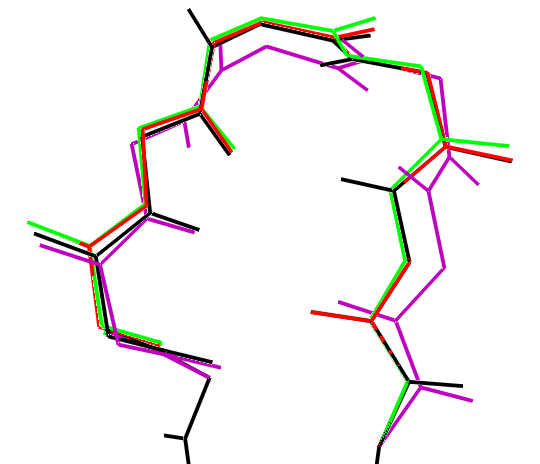
\includegraphics[width=2in,height=1.7in]{figures/cats_confs.png}\hspace{0.2in}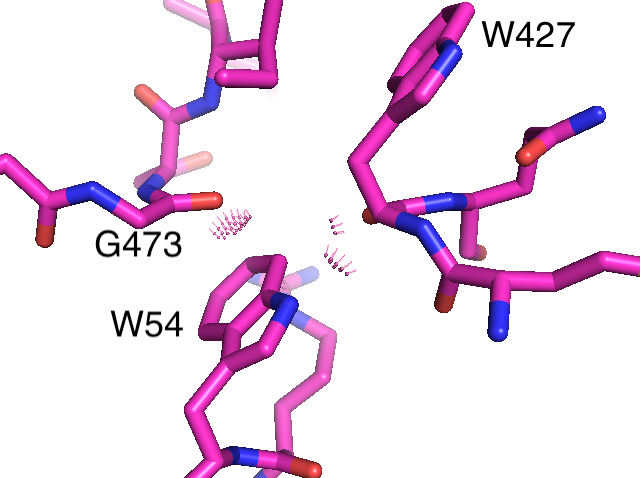
\includegraphics[width=2in,height=1.5in]{figures/w54_rigidBB_clashes.png}\hspace{0.2in}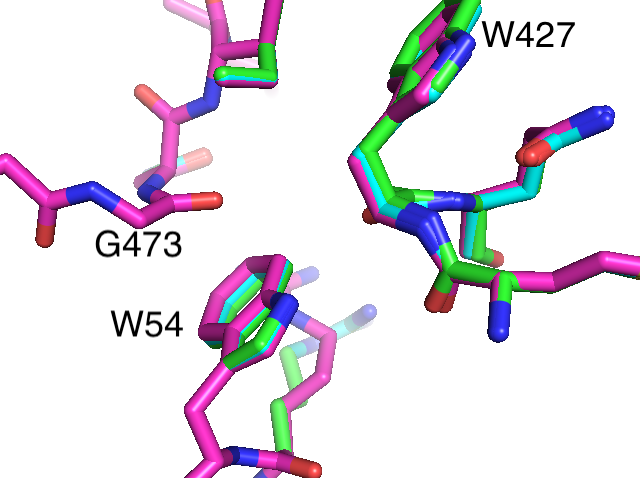
\includegraphics[width=2in,height=1.5in]{figures/w54_overlay.png}
\caption{Left: CATS allows systematic search over a voxel of backbone conformations in the vicinity of the wild-type backbone conformation (black).  The voxel is specified as box constraints on a novel set of backbone coordinates; conformations with one such coordinate moved to the edge of the voxel are shown in red and green, and a conformation with all such coordinates moved to the edge of the voxel is shown in purple.  See Fig. 1 of Ref.~\citen{CATS} for more details.  Middle: Rigid-backbone structural modeling of an experimentally effective mutant of anti-HIV gp120 antibody VRC07 showed unavoidable steric clashes between Trp 54 of VRC07 and Trp 427 and Gly 473 of gp120 (purple).  Right: CATS explained the experimentally observed activity by finding a new backbone conformation that resolved these clashes (green; overlaid with clashing rigid-body backbone (purple) and backbone conformation computed with the older DEEPer algorithm (blue)).  DEEPer reduced the clashes somewhat using backrub motions~\cite{backrub}, but they were still significant after the backrubs.  See Fig. 3 of Ref.~\citen{CATS} for more details.   Portions of this figure were reprinted with permission from Ref.~\citen{CATS}.  }
\label{fig:cats}
\end{figure}

This flexibility is enabled by the CATS algorithm~\cite{CATS} (Fig.~\ref{fig:cats}).  CATS uses a new parameterization of backbone conformational space, along with the voxel framework that {\sc osprey} has always included.  It is equivalent to searching over all changes in backbone dihedrals ($\phi$ and $\psi$) subject to keeping the protein conformation constant outside of a specified flexible region. CATS includes an efficient Taylor series-based algorithm for computing atomic coordinates from its new degrees of freedom, enabling efficient energy minimization.  Unlike previous protein design algorithms with backbone flexibility, CATS routinely finds backbone motions on the order of an angstrom (in RMSD with respect to the wildtype backbone) while still performing a comprehensive search of its backbone conformation space.  In Ref.~\citen{CATS}, we have shown that backbone flexibility as modeled by CATS is sometimes critical for avoiding nonphysical steric clashes (Fig.~\ref{fig:cats}B,C) and often affects energetics significantly.  For example, mutating residue 54 of the antibody VRC07 to tryptophan improves its binding to its antigen (HIV surface protein gp120)~\cite{VRC07_enhance}, but a design to recapitulate this mutation found it to be blocked by a steric clash unless CATS was used to find a backbone motion that escapes the clash~\cite{CATS}.  In this design, CATS significantly outperformed a provable search over backrub~\cite{backrub} motions, which are also available in \osprey~\cite{BRDEE,DEEPer}.  

CATS is intended to be run as part of the flexibility model for {\sc osprey}'s other algorithms, yielding efficient calculations with continuous flexibility in both the sidechains and the backbone. {\sc osprey}'s convenient interface allows a user to add CATS flexibility to a design merely by specifying the start and end points of the backbone segment to be made flexible.  

\def\as{\textit{$A^*$}\xspace}
\def\ks{\textit{$K^*$}\xspace}
\def\ka{\textit{$K_a$}\xspace}
\def\bbks{\textit{BBK$^*$}\xspace}

\subsection{\bbks: Efficiently computing the tightest binding sequences from a combinatorially large number of binding partners}

\bbks improves upon the \ks algorithm~\cite{}, which uses dead-end elimination pruning~\cite{} followed by \as~\cite{} gap-free conformation enumeration to provably approximate the association constant, \ka, as the ratio of $\varepsilon$-approximate partition functions between the bound and unbound states of a protein-ligand complex. Importantly, each partition function ratio, called a \ks \emph{score}, is provably accurate to the the biophysical \emph{input model}~\cite{}. This model defines the set of allowed amino acid mutations (i.e.~the \emph{sequence space}), structural search space (i.e.~the input structures, and allowed protein flexibility), the optimization objective (e.g.~design for binding affinity), and the energy function~\cite{}. \ks efficiently approximates \ka by using provable guarantees to compute the ensemble of most probable, low-energy conformations and discard higher energy, rarely populated conformations in the protein or ligand. Although \ks is considerably more efficient than exhaustive conformation enumeration for all possible sequences, \ks and all previous provable ensemble-based algorithms~\cite{} are \emph{single-sequence} algorithms, which explicitly consider every allowed sequence. The empirical and asymptotic runtime complexity of single-sequence algorithms is linear in the number of possible sequences, and therefore exponential in the number of mutable residues. As the number of mutable residues increases, the number of possible sequences increases exponentially. Therefore, designs with many mutable residues rapidly become intractable when using single-sequence algorithms. To manage the combinatorial explosion of the sequence space, \ks uses its inter-mutation pruning filter to prune sequences whose \ks scores provably cannot be within a user-specified factor of the best sequence encountered thus far. Nevertheless, inter-mutation pruning is applied only \emph{after} \ks initiates binding affinity computation.

~\cite{BBK*}

\jeff{Do we want to mention MPLP here?}
%etc

\section{Performance enhancements in version 3}
\osprey 3.0's code has been heavily optimized to improve single-threaded performance relative to the previous version, \osprey 2.2~\cite{COMETS}. Two main areas have received the most attention, and the most improvement in performance, so far: \as search speed, and conformation minimization speed.

\osprey uses the \as search algorithm~\cite{DEE/A*} to perform its combinatorial search over sequence and conformational space.  The performance of \as search in \osprey depends mostly on the size of the conformation space of the design. More mutable and flexible residues create a larger conformation space which must be searched systematically to find the lowest-energy conformations while preserving guarantees on solution quality, and hence the search requires more time. Search time is also dependent on the speed at which we can evaluate the scoring functions on \as nodes. Optimizations in \osprey 3.0 have dramatically increased the \as node scoring speed, mainly by caching the results of expensive computations and reusing them at different nodes. Many intermediate values used by the \as scoring functions need only be computed once per design. This reduces the cost of node scoring by roughly an order of magnitude. We can also score child nodes differentially against their parent nodes to speed up node scoring. Caching intermediate values during the parent node scoring and using them to simplify child node scoring yields roughly another order of magnitude speedup in \as node scoring. %\jeff{trying to be concise here, hopefully we don't need the mathematical details of these \as scoring functions?}

\osprey 3.0 also includes optimizations to improve the performance of forcefield evaluation and conformation minimization. Conformation minimization is typically the bottleneck in \osprey calculations with continuous flexibility~\cite{minDEE,iMinDEE,DEEPer,CATS}.  The code in \osprey 3.0 that evaluates forcefield energies for a protein conformation has been heavily optimized, although speed gains here over \osprey2 are modest (roughly two-fold), since the original code was already well-optimized in this area. Much larger performance increases were gained by caching forcefield parameters and lists of atom pairs between different conformations to be minimized and yielded roughly a 10-fold increase in speed. \osprey 3.0 also increases performance by only evaluating forcefield terms involving mutable and/or flexible residues in a design, since interaction energies between other residues will be exactly the same across all sequences and conformations.  Since most designs only model a minority of the residues in a protein as flexible, this can be a substantial improvement. 

Combined together, these optimizations to single-threaded performance made \osprey 3.0 about 425-fold faster than \osprey 2.2 on a small benchmark sidechain packing problem involving a 114-residue fragment of PDZ3 domain of PSD-95 protein complexed with a 6-residue peptide ligand (PDB ID: 1TP5) and consisting of six continuously flexible residues.  On an Intel Xeon E5-2640 v4 CPU, \osprey 2.2 took 49.5 minutes to run this benchmark, but \osprey 3.0 finished in 7.0 seconds.  

A major performance bottleneck of \osprey designs with continuous flexibility is minimizing protein conformations and conformation fragments. Since the space of possible conformations in a design grows exponentially with the number of flexible and mutable residues, the number of conformations that must (in the worst-case) be enumerated to find the GMEC or to approximate the Boltzmann-weighted partition function grows exponentially as well. Since all enumerated conformations must be subsequently minimized to compute their energies, and minimization is a relatively expensive operation, the bulk of a design's runtime can be spent on energy minimization of conformations. Therefore, improvements to the speed of energy minimization (an operation that is called an exponential number of times) can have a dramatic impact on \osprey runtimes.

Much work has been done in the past to optimize \osprey for execution on CPUs, particularly highly multi-core CPUs and even networked clusters of CPU-powered servers~\cite{minBounds_DACS,cloud_OSPREY}. However, modern GPU hardware enables high-performance computation at a fraction of the cost of large CPU clusters, mainly due to the huge video game industry that propels innovation in hardware design and drives down costs. \osprey3 includes GPU programs (called {\it kernels}) built using the CUDA framework that implements the forcefield calculations and local minimization algorithms used in protein redesign. We present performance results of these GPU kernels on various hardware platforms in Figure~\ref{fig:gpu}. Overall, on desktop-class machines, GPU hardware improves minimizations speeds over multi-core CPUs by roughly 12-fold for sufficiently large molecules. On server-class machines, a single GPU is merely about 2.6-fold faster than dual CPUs. These large machines can house more GPUs than CPUs though, so a fully-provisioned server with 4 or even 8 GPUs would likely greatly outperform 2 or even 4 CPUs. Laptop-class GPUs, however, do not appear to be powerful enough to offer any advantages over traditional CPU computing in \osprey3.

Modern GPU architectures offer thousands of parallel hardware units for calculations, compared to the tens of parallel hardware units in modern CPU architectures. The performance results of the current incarnation of \osprey's GPU kernels indicate that current minimization speeds on GPUs have only begun to scratch the surface of what is possible, particularly for molecules with a small number of atom pairs. It is incredibly likely that future versions of these GPU kernels will offer significantly higher performance on the same hardware -- perhaps allowing minimization speeds many times faster than today's GPU kernels.

\begin{figure}\label{fig:gpu}
\center
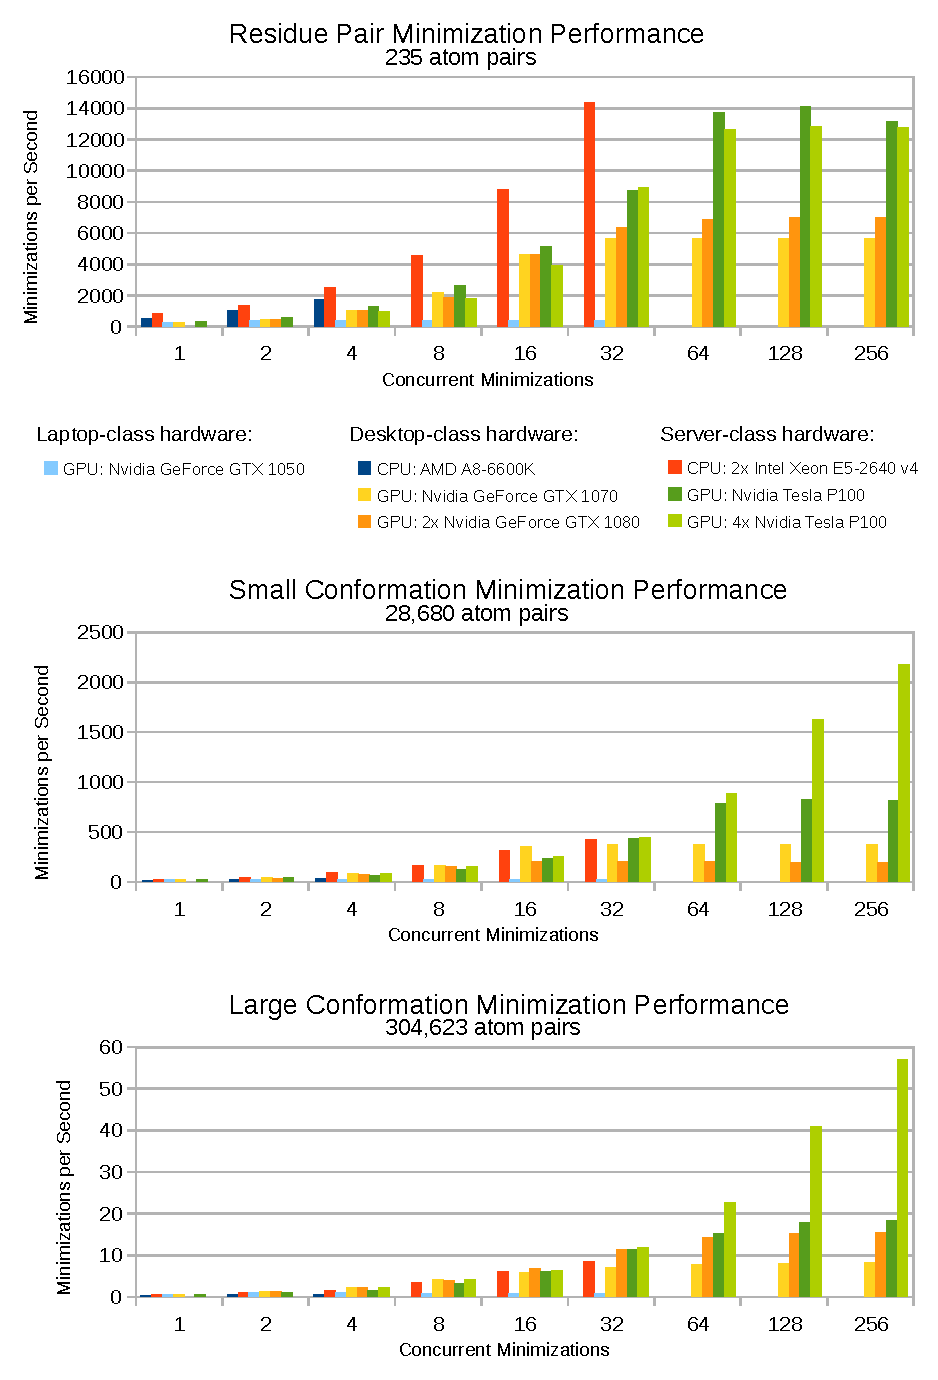
\includegraphics[width=4in]{figures/gpu.pdf}
\caption{Benchmarks for protein conformation minimization in \osprey3 for various hardware platforms and for molecules of varying size. From smallest to largest: {\bf (top)} a single residue pair used in energy matrix computations, {\bf (middle)} a full protein conformation with a single flexible residue, {\bf (bottom)} a full protein conformation with 20 flexible residues. For CPU hardware, concurrent minimizations correspond to CPU threads. For GPU hardware, concurrent minimizations correspond to {\it streams} defined by the CUDA framework. Faster minimization speeds correspond with faster \osprey runtimes.}
\end{figure}


\section{Python scripting improves ease-of-use}

One of the most visible additions to \osprey3 is the Python application programming interface (API), which allows fine-grained control over design parameters while also presenting a very easy-to-use experience. \osprey3 still supports a command-line interface with configuration files for backwards compatibility, but new development will be focused mostly on the new Python interface. \jeff{Is this even true? Not entirely sure...}

The \osprey3 distribution contains a Python module which can be installed using the popular package manager {\sc pip}. Once installed, using \osprey3 is as easy as writing a python script. High-performance computations are still performed in the Java virtual machine to give the fastest runtimes, so Java is still required to run \osprey3, but communication between the Python enviroment and the Java environment is handled behind-the-scenes, and \osprey3 still looks and feels like a regular Python application.

See Figure~\ref{fig:python} for a complete example of a Python script that performs a very simple design using \osprey3.

\begin{figure}\label{fig:python}
{\fontfamily{pcr}
	\lstinputlisting[language=Python]{figures/findGMEC.py}
}
\caption{A Python script that performs a very simple design in \osprey3.}
\end{figure}



\bibliographystyle{plain}
\bibliography{references}


\end{document}  